\documentclass[a4paper,letterpaper]{article}
 \usepackage{float}
 \usepackage[margin=2.54cm]{geometry}
 \usepackage{graphicx}
 \usepackage{anysize}
 \usepackage{lipsum}
 \usepackage{amsmath,amssymb,amsthm}
 \usepackage[utf8]{inputenc}
 \usepackage{multirow}
 \usepackage{csquotes}
 \usepackage[spanish]{babel}
 \usepackage{apacite}
 \usepackage{multicol}
 \usepackage{parskip}
 \usepackage{setspace}
 \doublespacing
\begin{document}
\begin{titlepage}
	\centering
	\vspace{3cm}
	{\scshape\Huge Trabajo de Mecánica de Fluidos \par}
	\vspace{3cm}
	\textbf\large\scshape{\par}
	\vspace{3cm}

	{\Large Vergara Pareja Gustavo\\Pacheco Berrio Jhosuea\\Petro Yanéz Edwin\par}
	\vspace{5cm}
	{\scshape\Large Programa de Ingeniería Mecánica \par}
	\vspace{1cm}
	{\scshape\Large Universidad de Córdoba\par}
	{\Large \today \par}
\end{titlepage}
\newpage
\tableofcontents
\newpage
\section*{Introducción}
\addcontentsline{toc}{section}{Introducción}
El presente proyecto tiene como objetivo principal aplicar los principios de flotabilidad y estabilidad en el diseño y construcción de un bote. La mecánica de fluidos es una rama fundamental de la física que estudia el comportamiento de los fluidos en reposo o en movimiento. En este caso, nos enfocaremos en la forma en que los fluidos interactúan con el bote y cómo se puede lograr que este flote y se mantenga estable en el agua.
\newline

Se responderán preguntas
como: ¿Cómo se diseñó el casco?, ¿Con qué materiales se construyó? y ¿Cuál es su finalidad?.
\newline
Para lograr este objetivo, se utilizarán principios de la física y la mecánica para describir
el movimiento del casco y se analizarán las fuerzas involucradas en su funcionamiento.
Además, se describirá el diseño mecánico de este, incluyendo los materiales utilizados
y las especificaciones técnicas.
\newpage
\section*{Objetivos}
\addcontentsline{toc}{section}{Objetivos}
\subsubsection*{Objetivo General}
\begin{itemize}
	\item Diseñar y construir el casco de un bote aplicando los principios de flotabilidad y estabilidad.
\end{itemize}
\subsubsection*{Objetivos Específicos}
\begin{itemize}
	\item Analizar y aplicar los conceptos teóricos de la mecánica de fluidos para comprender los principios de flotabilidad y estabilidad en el diseño de embarcaciones.
	\item Diseñar un bote que cumpla con los criterios de flotabilidad y estabilidad, considerando la ubicación del centro de gravedad, el centro de flotación y la forma del casco.
	\item Evaluar experimentalmente el desempeño del bote en términos de flotabilidad y estabilidad, realizando pruebas en condiciones controladas de agua y registrando datos relevantes como la inclinación, el desplazamiento y la capacidad de carga del bote.
\end{itemize}
\newpage

\section*{Teoría Relacionada}
\addcontentsline{toc}{section}{Teoría Relacionada}
\subsubsection*{Principio de Arquímedes}
\setlength{\parindent}{18pt} 
Los barcos flotan, gracias los aportes realizados por Arquímedes (Principio de Arquímedes);
 la cual establece que cuando un objeto se sumerge total o parcialmente en un líquido, 
 éste experimenta un empuje hacia arriba igual al peso del líquido desalojado;
dicha fuerza es vertical y está dirigida hacia arriba. El Empuje es igual al peso del volumen de líquido desplazado, y 
está aplicado en un punto denominado centro de empuje, que coincide con el centro de gravedad del objeto, 
cuando éste se encuentra en reposo (Redín Muñoz, 2007a).
$$E=V_{c} \cdot \gamma $$

\subsubsection*{Principio de Arquímedes}





\newpage
\section*{¿Qué se hizo?}
\addcontentsline{toc}{section}{¿Qué se hizo?}
El objetivo de este proyecto fué estudiar el movimiento del casco de un bote y realizar cálculos empíricos
de su flotabilidad, estabilidad y análisis de fuerzas. En la práctica, se construyó el casco de un barco a escala y se realizaron experimentos para medir. \begin{itemize}
	\item El centro de flotabilidad.
	\item El metacentro
	\item
\end{itemize}
\section*{Materiales y métodos}
\addcontentsline{toc}{section}{Materiales y métodos}
Los materiales utilizados para el desarrollo de este casco fueron:
\begin{itemize}
	\item Madera
	\item Pintura
	\item Marcadores
	\item Resina
	\item
	\item
	\item
\end{itemize}
\newpage
\section*{Contenido y Resultados}
\addcontentsline{toc}{section}{Contenido y Resultados}
Para el desarrollo de este proyecto, hicimos una búsqueda exhaustiva de modelos e ideas para construir el casco del barco:
\begin{figure}[H]
	\centering
	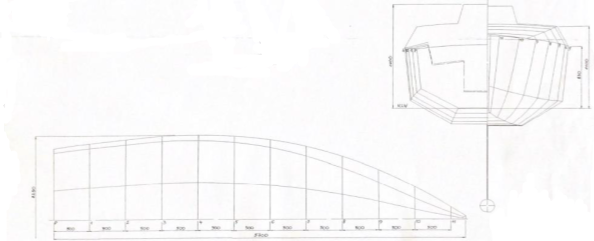
\includegraphics[width=1 \textwidth]{imgbarcoplano.png}
	\caption{ Planos oficiales ClassGlobe 5.80.}
	\label{fig:imagen}
\end{figure}
\begin{itemize}
	\item A continuación, comenzamos a construir el casco del barco.
\end{itemize}
\begin{figure}[H]
	\centering
	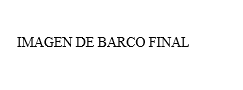
\includegraphics[width=0.5\textwidth]{imgbarcofinal.png}
	\caption{Toma de datos}
	\label{fig:imagen1}
\end{figure}
\begin{itemize}
	\item Luego de esto, pasamos a hacer mediciones y cálculos empíricos:
\end{itemize}
\begin{figure}[H]
	\centering
	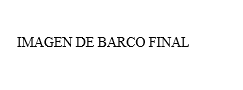
\includegraphics[width=0.8\textwidth]{imgbarcofinal.png}
	\caption{Barco con los criterios solicitados}
	\label{fig:imagen2}
\end{figure}
\begin{itemize}
	\item Análisis del barco
\end{itemize}
\begin{figure}[H]
	\centering
	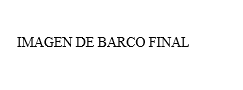
\includegraphics[width=0.8\textwidth]{imgbarcofinal.png}
	\caption{Carga máxima, centro de gravedad y flotabilidad...}
	\label{fig:imagen3}
\end{figure}
\newpage
Con SolidWorks Simulation, es posible realizar análisis de elementos finitos (FEA) para determinar las tensiones, deformaciones y factores de seguridad en la herramienta de corte y otras piezas importantes de la máquina.
Por otro lado, con SolidWorks Motion, es posible simular el movimiento de la máquina y su comportamiento dinámico bajo diferentes condiciones de carga.
\newline
A continuación calcularemos:

\begin{itemize}
	\item Velocidad
	      \newline
	      $$v=\frac{y}{t}=\frac{0.1m}{1s}=10cm/s$$
	\item Aceleracion
	      \newline
	      La aceleración de las cabinas sera igual a 0, ya que por la primera Ley de Newton, estos cuerpos
	      estan bajo velocidad constante.
	\item Tensión
	      \newline
	      Podemos calcular fuerza de tensión en los cables que sostienen las cabinas. Para hacer esto, podemos usar la segunda ley de Newton, que establece que la fuerza neta sobre un objeto es igual a su masa multiplicada por su aceleración. En este caso, la aceleración de las cabinas es cero, por lo que la fuerza neta es cero. Por lo tanto, la suma de las fuerzas en cada cabina debe ser igual a cero. Podemos escribir esto como:
	      \newline
	      $$F_{T}-\left ( m_{1}*g \right )-\left ( m_{2}*g \right )=0$$
	      $$F_{T}=\left ( 0.04kg*9.81\frac{m}{{s}^2} \right )+\left ( 0.04kg*9.81\frac{m}{{s}^2} \right )=0.8N$$
	\item Potencia
	      $$W=2T\cdot v=\left ( 0.8N \right )\left ( 0.1m/s \right )=0.08W$$
	\item Velocidad angular del eje:
	      \newline
	      Podemos calcular la velocidad angular del eje utilizando la fórmula:
	      \newline
	      $$w = v/r$$
	      $$w =\left ( 0.1m/s \right )/\left ( 0.02m \right )=5 rad/s$$
\end{itemize}
\section*{Conclusiones}
\addcontentsline{toc}{section}{Conclusiones}
En conclusión, el proyecto de diseño y construcción de un bote basado en los principios de flotabilidad y estabilidad es una oportunidad para aplicar los conocimientos teóricos de la mecánica de fluidos de manera práctica y significativa. A lo largo del proyecto, se han abordado conceptos clave como el principio de Arquímedes, el centro de flotación, la estabilidad y la resistencia hidrodinámica.
El diseño y construcción de un bote que cumpla con los principios mencionados requiere un enfoque integral que considere tanto los aspectos teóricos como los prácticos. Se han explorado conceptos teóricos fundamentales y se han aplicado en la práctica a través de la construcción del bote y la evaluación experimental de su desempeño en términos de flotabilidad y estabilidad.
Este proyecto ha permitido comprender la relación entre la teoría de la mecánica de fluidos y su aplicación práctica en el diseño y construcción de embarcaciones. Estos conocimientos adquiridos son valiosos tanto en el ámbito académico como en el profesional, ya que la mecánica de fluidos juega un papel fundamental en numerosas disciplinas relacionadas con el diseño


\newpage
\section*{}
\bibliographystyle{apacite}
\nocite{*}
\bibliography{referenciados}
\end{document}